\section{Różne parametry układu i wartości zadane}
%TODO: jakieś porównanie
\begin{figure}[p]
    \centering
	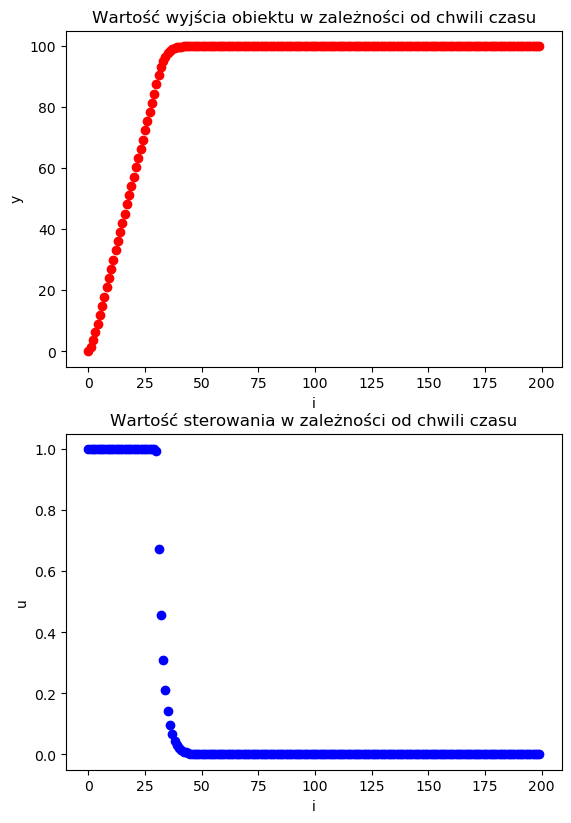
\includegraphics[width=\textwidth]{A_[0.1, 0.2, 0.1, 0.2, 0, 0.5, 0.1, 1, 0, 0, 1, 0, 0, 0, 0, 1]}
	\caption{Nasycone sterowanie}
	\label{fig:saturated}
\end{figure}

\section{Różne parametry regulatora}
%TODO: Opis parametrów stałych
\begin{figure}[p]
    \centering
	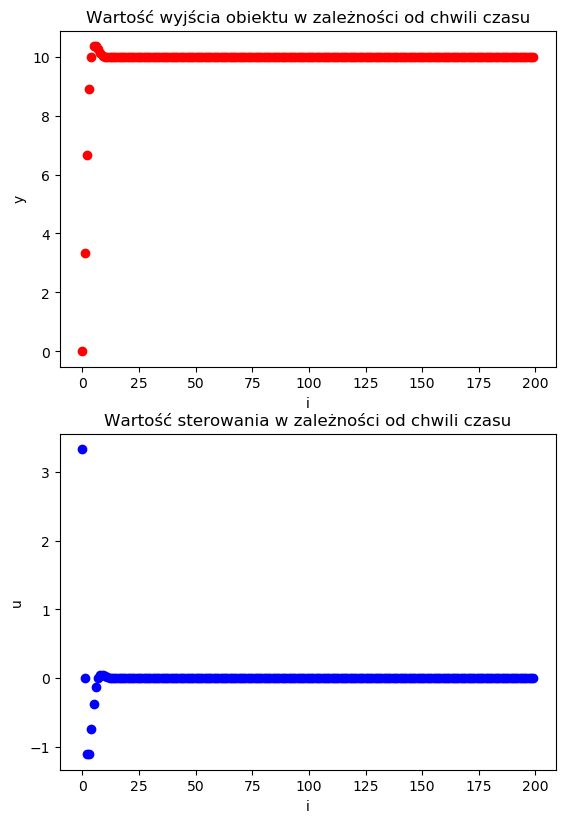
\includegraphics[width=\textwidth]{horizons_[3, 3]}
	\caption{Horyzont predykcji: 3, horyzont sterowań: 3}
	\label{fig:horizons_3_3}
\end{figure}

\begin{figure}[p]
    \centering
	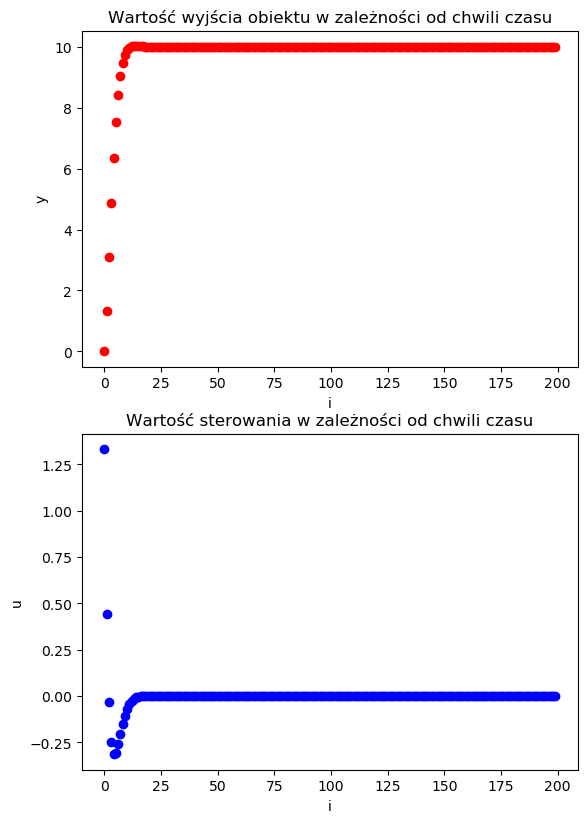
\includegraphics[width=\textwidth]{horizons_[5, 3]}
	\caption{Horyzont predykcji: 5, horyzont sterowań: 3}
	\label{fig:horizons_5_3}
\end{figure}

\begin{figure}[p]
    \centering
	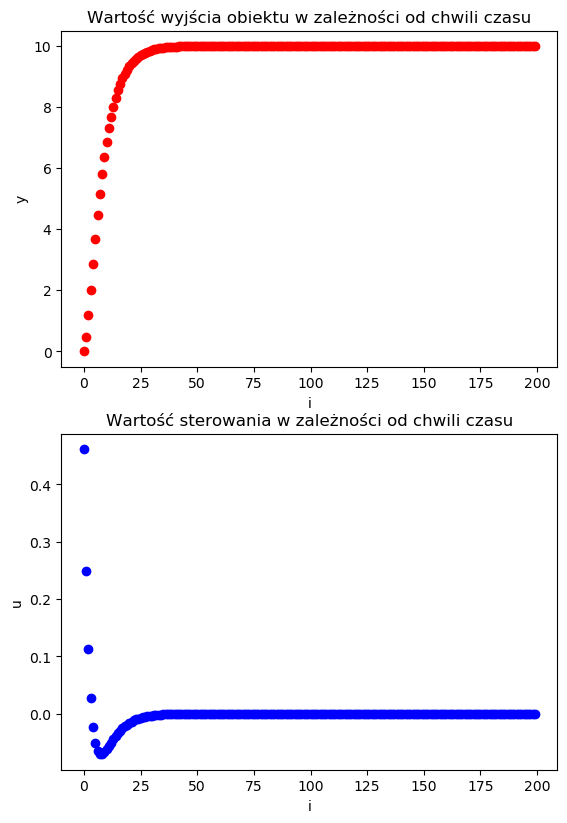
\includegraphics[width=\textwidth]{horizons_[10, 3]}
	\caption{Horyzont predykcji: 10, horyzont sterowań: 3}
	\label{fig:horizons_10_3}
\end{figure}

\begin{figure}[p]
    \centering
	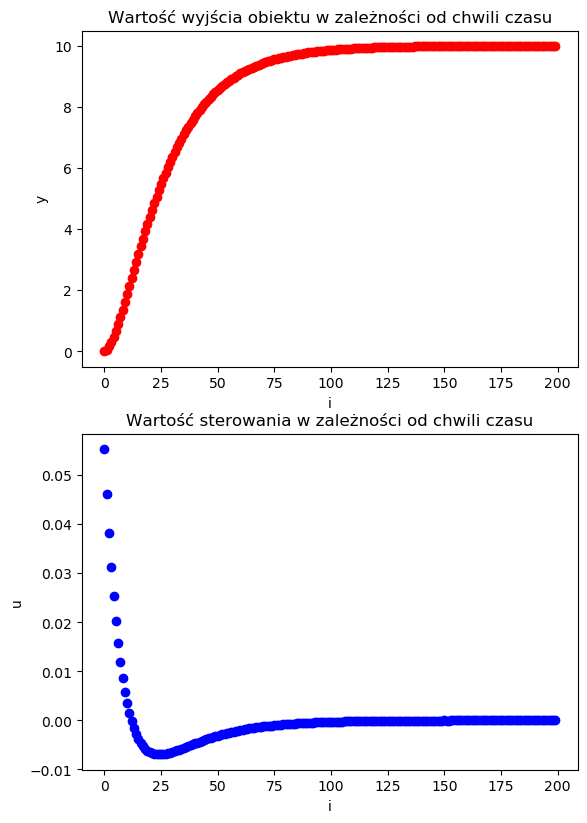
\includegraphics[width=\textwidth]{horizons_[15, 2]}
	\caption{Horyzont predykcji: 15, horyzont sterowań: 2}
	\label{fig:horizons_15_2}
\end{figure}

\begin{figure}[p]
    \centering
	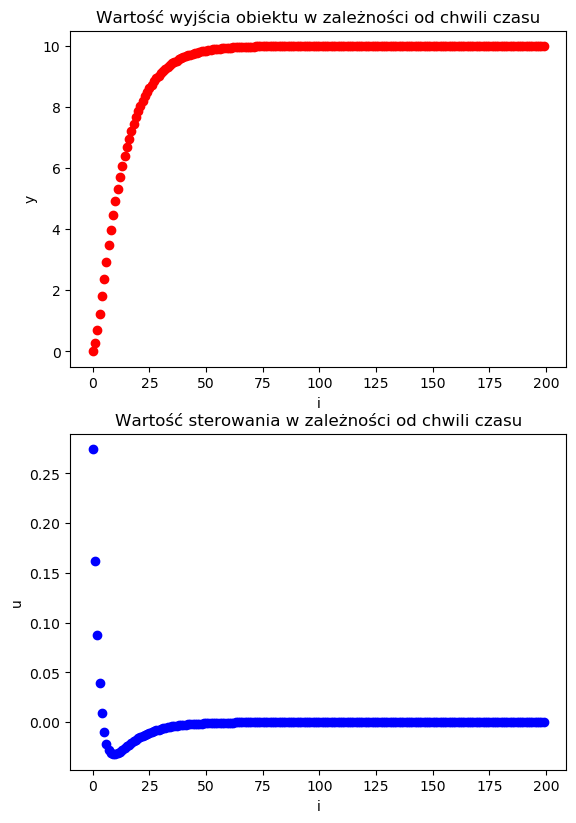
\includegraphics[width=\textwidth]{horizons_[15, 3]}
	\caption{Horyzont predykcji: 15, horyzont sterowań: 3}
	\label{fig:horizons_15_3}
\end{figure}

\begin{figure}[p]
    \centering
	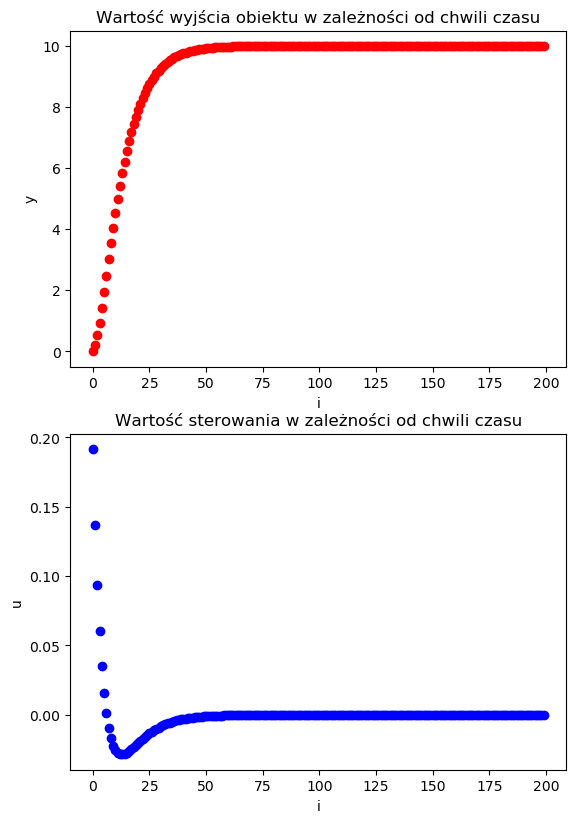
\includegraphics[width=\textwidth]{horizons_[15, 5]}
	\caption{Horyzont predykcji: 15, horyzont sterowań: 5}
	\label{fig:horizons_15_5}
\end{figure}

\begin{figure}[p]
    \centering
	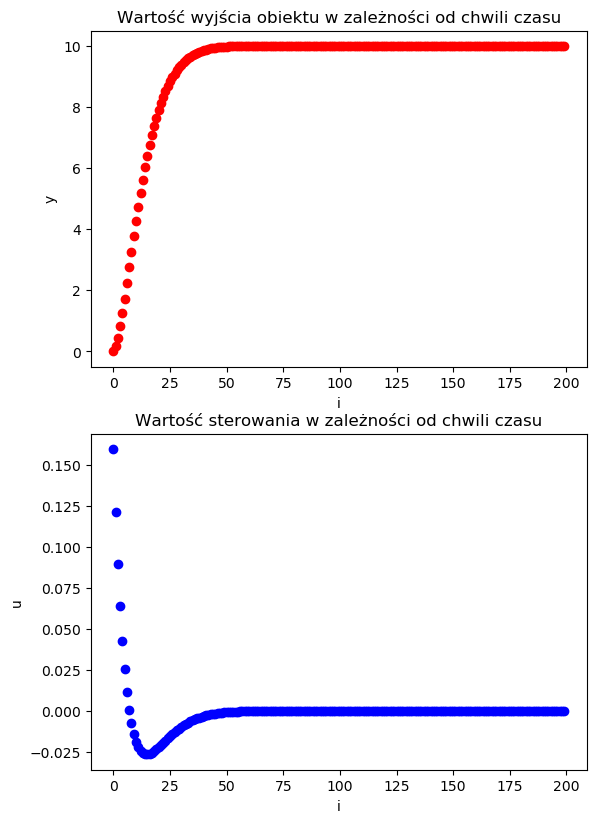
\includegraphics[width=\textwidth]{horizons_[15, 7]}
	\caption{Horyzont predykcji: 15, horyzont sterowań: 7}
	\label{fig:horizons_15_7}
\end{figure}

\begin{figure}[p]
    \centering
	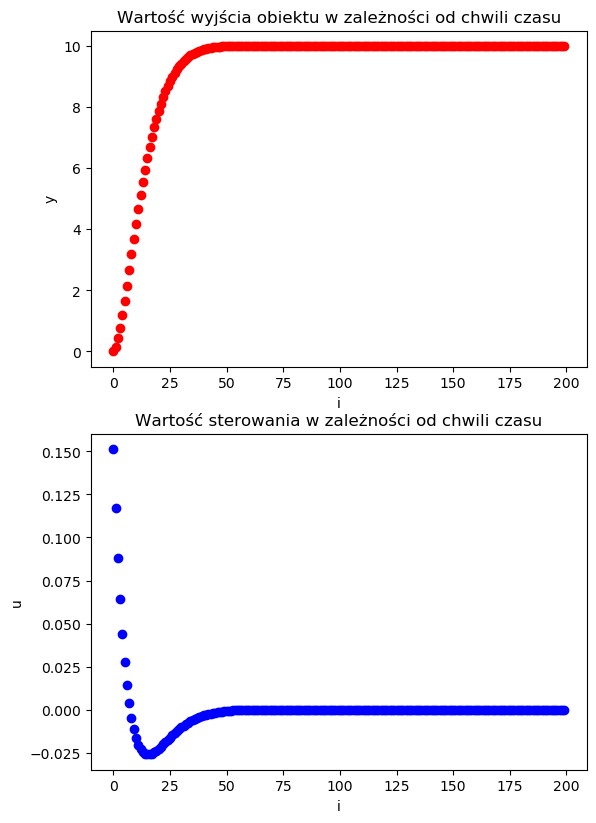
\includegraphics[width=\textwidth]{horizons_[15, 8]}
	\caption{Horyzont predykcji: 15, horyzont sterowań: 8}
	\label{fig:horizons_15_8}
\end{figure}

\begin{figure}[p]
    \centering
	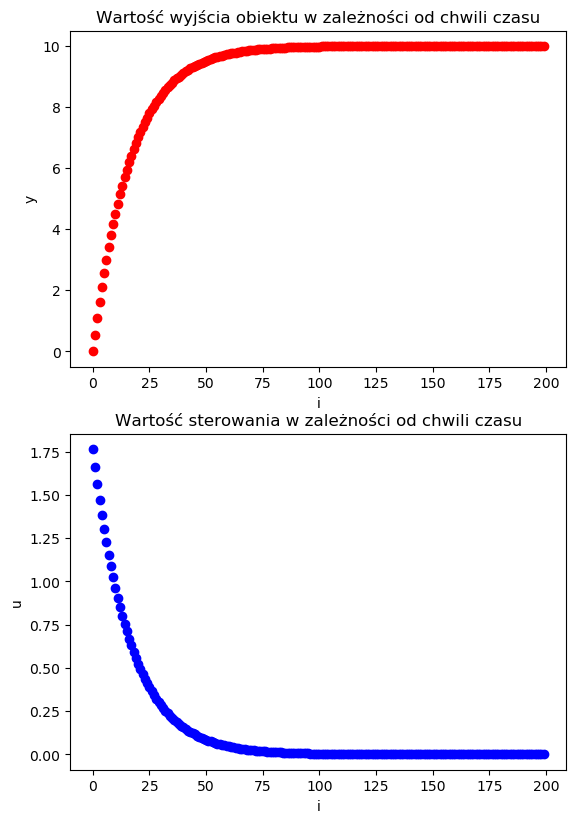
\includegraphics[width=\textwidth]{horizons_[30, 8]}
	\caption{Horyzont predykcji: 30, horyzont sterowań: 8}
	\label{fig:horizons_30_8}
\end{figure}